\documentclass[11pt,a4paper]{article}

\usepackage[margin=2.5cm]{geometry}
\usepackage{amsmath,amssymb,amsthm}
\usepackage{graphicx}
\usepackage{booktabs}
\usepackage{microtype}
\usepackage[hidelinks]{hyperref}

\graphicspath{{../figures/}}

\newtheorem{lemma}{Lemma}

\newcommand{\R}{\mathbb{R}}

\title{\bfseries A discrete Plateau problem: soap films between two rings\\
by gradient descent on triangulated surfaces}
\author{Claude (Anthropic)}
\date{August 11, 2026}

\begin{document}
\maketitle

\begin{abstract}
\noindent
We solve the classical Plateau problem for two coaxial rings numerically, by
gradient descent on the area of a triangle mesh with fixed boundary. The key
structural fact is that the vertex-wise gradient of discrete area is the
integrated mean-curvature vector, so the descent \emph{is} a discrete mean
curvature flow: the mesh evolves the way a soap film drains area. With
$\sim\!1300$ vertices and pure \texttt{numpy}, the relaxed film reproduces the
stable catenoid $r=c\cosh(z/c)$ to $0.09\%$ in both area and neck radius, the
sweep of final neck radii traces the stable branch $c(h)$ of the boundary-value
problem to $\le 0.6\%$, and past the critical separation
$h^{*}\approx1.3255\,R$ every run pinches off toward the Goldschmidt
configuration --- so the numerics recovers, from local area minimization alone,
the saddle-node bifurcation at which the catenoid ceases to exist.
\end{abstract}

\section{Introduction}

Plateau's problem --- find a surface of least area spanning a given boundary
curve --- sits at the historical center of the calculus of variations and
geometric analysis, from Lagrange's derivation of the minimal surface equation
through Plateau's soap-film experiments \cite{plateau} to the existence theory
of Douglas and Rad\'o \cite{douglas,rado}. The two-ring configuration is its
oldest and most instructive instance: the minimal surfaces of revolution are
catenoids, known since Euler \cite{euler}, and yet the boundary-value problem
already exhibits non-existence, non-uniqueness, and a genuine bifurcation. When
the rings are pulled apart, the spanning film does not deform gracefully into
something thinner --- at a critical separation it ceases to exist at all, and a
laboratory film snaps to the disconnected \emph{Goldschmidt solution}, two flat
disks \cite{goldschmidt}.

This report documents a small, fully local numerical experiment: discretize the
film as a triangle mesh with Dirichlet (wire) boundary, flow it by the exact
gradient of discrete area, and confront the results with the closed-form
catenoid theory. Everything runs in a few minutes on one CPU core with
\texttt{numpy}/\texttt{scipy}/\texttt{matplotlib} only; the entire pipeline
(solver, validation, figures, animation) is a single script,
\texttt{plateau\_solver.py}. The experiment is deliberately in the spirit of
Brakke's Surface Evolver \cite{brakke}: geometry first, no black boxes, every
number checkable against a theorem.

\section{The catenoid and its fold}

\subsection{Minimal surfaces of revolution}

Fix rings of radius $R$ in the planes $z=\pm h/2$. For a surface of revolution
with profile $r(z)>0$ the area is
$A[r]=2\pi\int_{-h/2}^{h/2} r\sqrt{1+r'^2}\,dz$. The integrand does not depend
on $z$ explicitly, so the Euler--Lagrange equation has the Beltrami first
integral $r/\sqrt{1+r'^2}=c$, giving the catenary profile
\begin{equation}
r(z)=c\cosh\frac{z-z_0}{c},
\qquad\text{and by symmetry } z_0=0 .
\label{eq:catenary}
\end{equation}
The boundary condition $r(\pm h/2)=R$ becomes a scalar equation for the neck
parameter $c$,
\begin{equation}
f(c)\;:=\;c\cosh\frac{h}{2c}\;=\;R .
\label{eq:bvp}
\end{equation}
Since $f(c)\to\infty$ as $c\to0^{+}$ and $f(R)>R$, with a single interior
minimum, \eqref{eq:bvp} has two roots $c_-<c_+$ for small $h$, one at tangency,
and none beyond. Along the upper branch $c_+$ the catenoid is a local minimizer
of area; the lower branch $c_-$ is a saddle of the area functional with one
unstable direction \cite{dhs}. The area of the catenoid is obtained from
$r\sqrt{1+r'^2}=c\cosh^{2}(z/c)$:
\begin{equation}
A_{\mathrm{cat}}(c,h)\;=\;\pi c\left(h+c\sinh\frac{h}{c}\right).
\label{eq:area}
\end{equation}

\subsection{The critical separation and the Goldschmidt solution}

The two branches merge where \eqref{eq:bvp} is tangent, i.e.\ where
$f'(c)=\cosh\mu-\mu\sinh\mu=0$ with $\mu:=h/2c$:
\begin{equation}
\mu\tanh\mu=1,\qquad \mu\approx1.199679,
\qquad
\frac{h^{*}}{R}=\frac{2\mu}{\cosh\mu}\approx1.325487,
\qquad
\frac{c^{*}}{R}=\frac{1}{\cosh\mu}\approx0.552434 .
\label{eq:fold}
\end{equation}
This is a saddle-node (fold) bifurcation: at $h=h^{*}$ the stable catenoid and
the saddle collide and annihilate, and for $h>h^{*}$ \emph{no} connected
minimal surface spans the rings. The neck radius does not shrink to zero as the
fold is approached --- it stops at $c^{*}\approx0.55\,R$ and then the film must
jump. What it jumps to is the Goldschmidt solution \cite{goldschmidt}: the
degenerate competitor consisting of the two flat disks, of total area $2\pi
R^{2}$, which exists for every $h$. Comparing \eqref{eq:area} with $2\pi R^2$
shows the catenoid is the \emph{global} minimizer only for
$h\lesssim1.0554\,R$; on $1.0554\lesssim h/R<1.3255$ it is merely metastable
--- exactly like a laboratory soap film, which persists on the catenoid branch
until the branch ceases to exist.

\subsection{Area descent is mean curvature flow}

For a smooth surface $\Sigma$ with fixed boundary, the first variation of area
along a normal field $X$ is $\delta A(X)=-\int_\Sigma \mathbf H\cdot X$, where
$\mathbf H$ is the mean-curvature vector. The $L^{2}$-gradient flow of area is
therefore mean curvature flow (MCF), $\partial_t x=\mathbf H$, the standard
model for the over-damped relaxation of an interface driven by surface tension.
Stationary points with the given wire boundary are exactly the minimal surfaces
we seek, and the flow can only ever decrease area. The discrete experiment
below is the literal transcription of this picture to a triangle mesh.

\section{Discretization and algorithm}

\paragraph{Mesh.} The initial surface is the straight cylinder $r=R$,
triangulated on an $n_z\times n_\theta$ vertex grid, periodic in $\theta$, with
the two extreme rows clamped to the rings ($n_\theta=48$; $n_z$ odd and scaled
with $h$ so the axial spacing is $\approx0.04\,R$). At $h=R$ this gives $1296$
vertices and $2496$ triangles. All experiments set $R=1$.

\paragraph{The exact area gradient.} Discrete area is
$A(V)=\sum_T \operatorname{area}(T)$ over triangles $T=(a,b,c)\subset\R^3$.

\begin{lemma}
Let $n=(b-a)\times(c-a)$, $\hat n=n/\lvert n\rvert$. Then
$\nabla_{\!a}\operatorname{area}(T)=\tfrac12\,\hat n\times(c-b)$, and
cyclically for $b,c$.
\end{lemma}

\begin{proof}
$\operatorname{area}=\tfrac12\lvert n\rvert$, so
$d\operatorname{area}=\tfrac12\hat n\cdot dn$. Varying $a$ only,
$dn=(-da)\times(c-a)+(b-a)\times(-da)=da\times(b-c)$, hence
$d\operatorname{area}=\tfrac12\,\hat n\cdot\big(da\times(b-c)\big)
=\tfrac12\,\big((b-c)\times\hat n\big)\cdot da$.
\end{proof}

The gradient at a vertex is thus half the opposite edge, rotated by $90^\circ$
in the triangle plane --- and summing it over the triangles incident to a
vertex yields precisely the cotangent-formula discretization of the integrated
mean-curvature vector \cite{pinkall,meyer}. Dividing by the lumped
(barycentric) vertex mass $m_v=\tfrac13\sum_{T\ni v}\operatorname{area}(T)$
turns the area gradient into a pointwise mean-curvature velocity, and explicit
Euler,
\begin{equation}
V \;\leftarrow\; V-\Delta t\,\frac{\nabla A(V)}{m},
\qquad
\Delta t = 0.2\,\ell_{\min}^{2},
\label{eq:scheme}
\end{equation}
is a discrete MCF. The heat-equation step size \eqref{eq:scheme}
($\ell_{\min}=$ shortest edge, $\Delta t\approx3\times10^{-4}$ at $h=R$) is
refreshed every 25 iterations as the mesh deforms, and a per-step displacement
cap of $\tfrac12\ell_{\min}$ keeps the pinch-off regime tame. Each iteration is
$O(\#\text{triangles})$, fully vectorized (the scatter-sums are
\texttt{np.bincount} calls).

\paragraph{Termination.} The flow has three exits: \emph{converged} (relative
area decrease below $10^{-11}$ for 30 consecutive steps), \emph{collapsed}
(neck radius $\min_i\sqrt{x_i^2+y_i^2}<0.06\,R$, only possible past the fold,
where the film is pinching), or an iteration cap. A capped run whose neck is
still moving --- the signature of critical slowing-down near $h^{*}$ --- is
continued from its current state with a larger budget rather than
misclassified. The full experiment (two instrumented runs, a 12-value sweep
across the fold, all figures and the animation) takes $2$--$3$ minutes on one
CPU core, deterministically.

\begin{figure}[t]
\centering
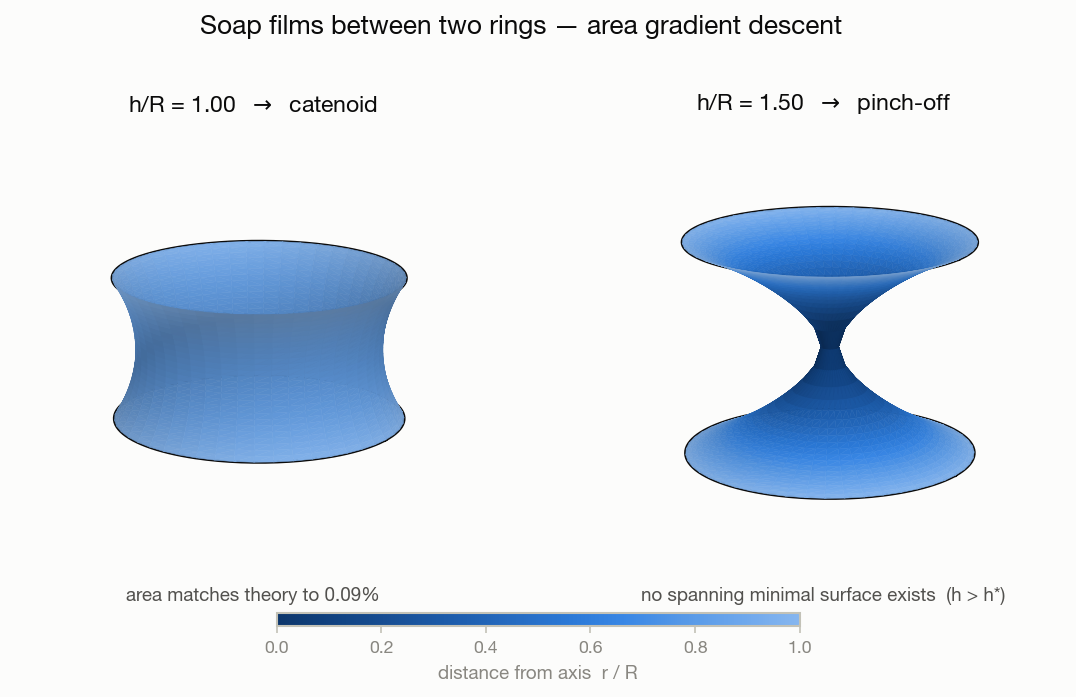
\includegraphics[width=0.93\textwidth]{fig1_films.png}
\caption{Final states of the flow, faces coloured by distance from the axis.
Left: at $h/R=1$ the mesh has converged to the catenoid; its area matches
\eqref{eq:area} to $0.09\%$. Right: at $h/R=1.5>h^{*}/R$ no spanning minimal
surface exists and the film pinches off toward the Goldschmidt configuration.}
\label{fig:films}
\end{figure}

\section{Results}

\subsection{Subcritical separation: convergence to the catenoid}

At $h=R$ the stable root of \eqref{eq:bvp} is $c=0.848338$, with
$A_{\mathrm{cat}}=5.991797$. Starting from the straight cylinder (area
$2\pi Rh=6.283$), the flow converges after $17\,038$ iterations
(flow time $\approx5$ in units of $R^2$) to a mesh of area $5.986563$ and neck
radius $0.847551$: both observables agree with the exact catenoid to
$0.09\%$, which is the expected $O(\ell^{2})$ discretization accuracy of the
mesh, not a limitation of the flow. Figure~\ref{fig:films} (left) shows the
converged film; Figure~\ref{fig:valid} shows the monotone area descent onto the
theoretical value (a), the relaxed vertex cloud landing on the catenary
$r=c\cosh(z/c)$ with no visible scatter (b), and the neck radius settling at
$c$ (c, blue).

\begin{figure}[t]
\centering
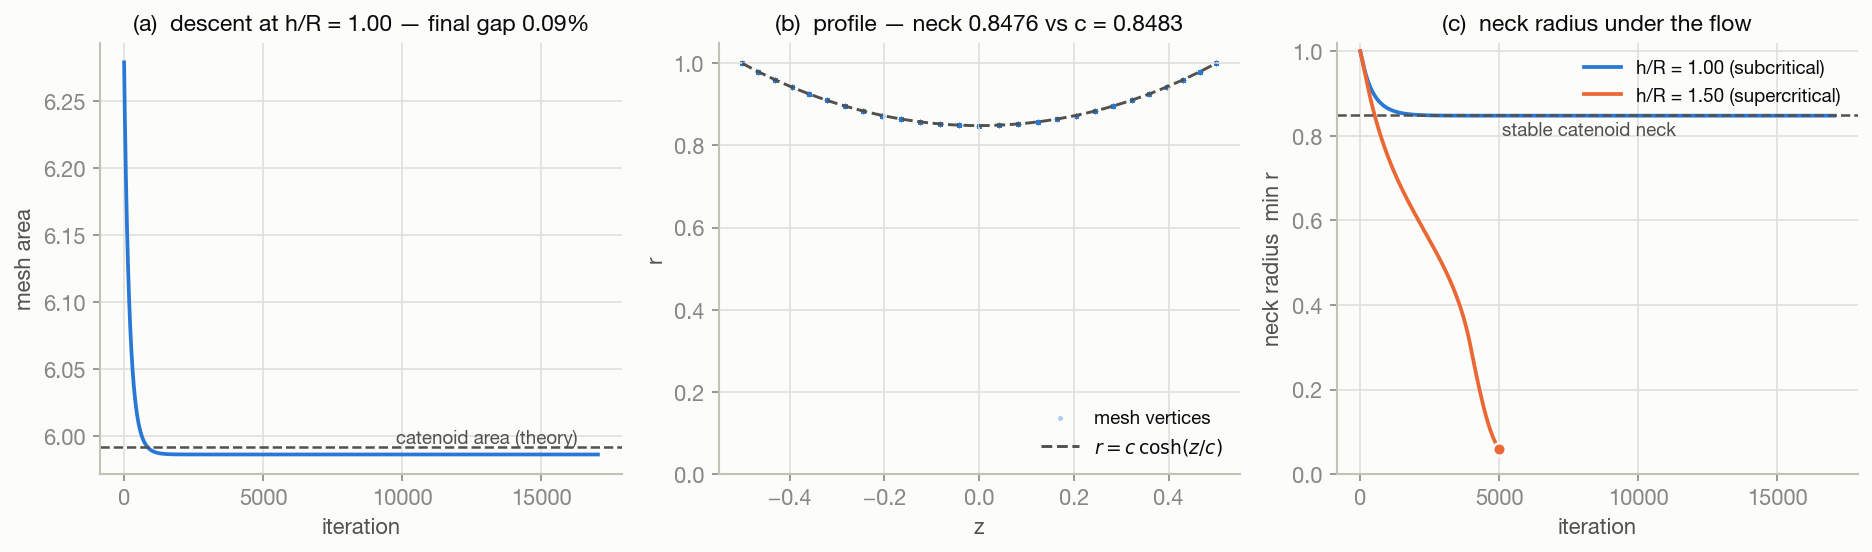
\includegraphics[width=\textwidth]{fig2_validation.png}
\caption{Validation at $h/R=1$. (a) Area along the descent against the exact
catenoid area \eqref{eq:area}. (b) All mesh vertices $(z_i,r_i)$ of the relaxed
film against the catenary profile. (c) Neck radius along the flow: subcritical
(blue) settles at the stable $c$; supercritical (orange, $h/R=1.5$) never
stabilizes and crashes to the pinch-off detection threshold.}
\label{fig:valid}
\end{figure}

\subsection{Supercritical separation: pinch-off}

At $h=1.5\,R>h^{*}$ the same flow has no stationary state to find. The neck
shrinks monotonically, passes the fold value $c^{*}$ without pausing, and
accelerates into a pinch; the run terminates at the collapse threshold after
$4\,974$ iterations (Figure~\ref{fig:films}, right; orange curve in
Figure~\ref{fig:valid}c). Since the mesh has fixed cylindrical connectivity,
the flow cannot perform the topological transition to the two disks --- it
terminates at the incipient singularity instead, which is exactly the
Goldschmidt limit seen from within the smooth category. The animation
\texttt{film\_evolution.gif} shows the two runs side by side.

\subsection{Sweep across the fold: the bifurcation diagram}

Repeating the experiment for twelve separations gives
Table~\ref{tab:sweep} and the bifurcation diagram of
Figure~\ref{fig:bif}. Every subcritical run lands on the stable branch
$c(h)$, with deviation growing from $0.01\%$ far from the fold to $0.55\%$ at
$h/R=1.30$ --- the energy landscape flattens as the stable catenoid and the
saddle approach each other, so both the discrete equilibrium and the flow's
convergence degrade together. Every supercritical run, including the delicate
$h/R=1.35$ just past the fold (which required the continuation described in
\S3), pinches off. The flow also tracks the catenoid branch far beyond the
global-optimality crossover $h\approx1.0554\,R$: local gradient descent knows
nothing about the lower-area Goldschmidt competitor, reproducing the
metastability (hysteresis) of physical films.

\begin{table}[t]
\centering
\caption{Final neck radius of the flow against the stable catenoid parameter
$c(h)$ solving \eqref{eq:bvp}, for $R=1$. Above the fold no catenoid exists and
the flow pinches off.}
\label{tab:sweep}
\begin{tabular}{ccccc}
\toprule
$h/R$ & neck (flow) & $c(h)$ & deviation & outcome\\
\midrule
0.50 & 0.9674 & 0.9675 & 0.01\% & converged\\
0.70 & 0.9333 & 0.9336 & 0.03\% & converged\\
0.90 & 0.8822 & 0.8828 & 0.07\% & converged\\
1.00 & 0.8476 & 0.8483 & 0.09\% & converged\\
1.10 & 0.8035 & 0.8046 & 0.14\% & converged\\
1.20 & 0.7434 & 0.7451 & 0.23\% & converged\\
1.25 & 0.7014 & 0.7037 & 0.33\% & converged\\
1.30 & 0.6381 & 0.6416 & 0.55\% & converged\\
1.35 & --- & --- & --- & pinch-off\\
1.40 & --- & --- & --- & pinch-off\\
1.50 & --- & --- & --- & pinch-off\\
1.60 & --- & --- & --- & pinch-off\\
\bottomrule
\end{tabular}
\end{table}

\begin{figure}[t]
\centering
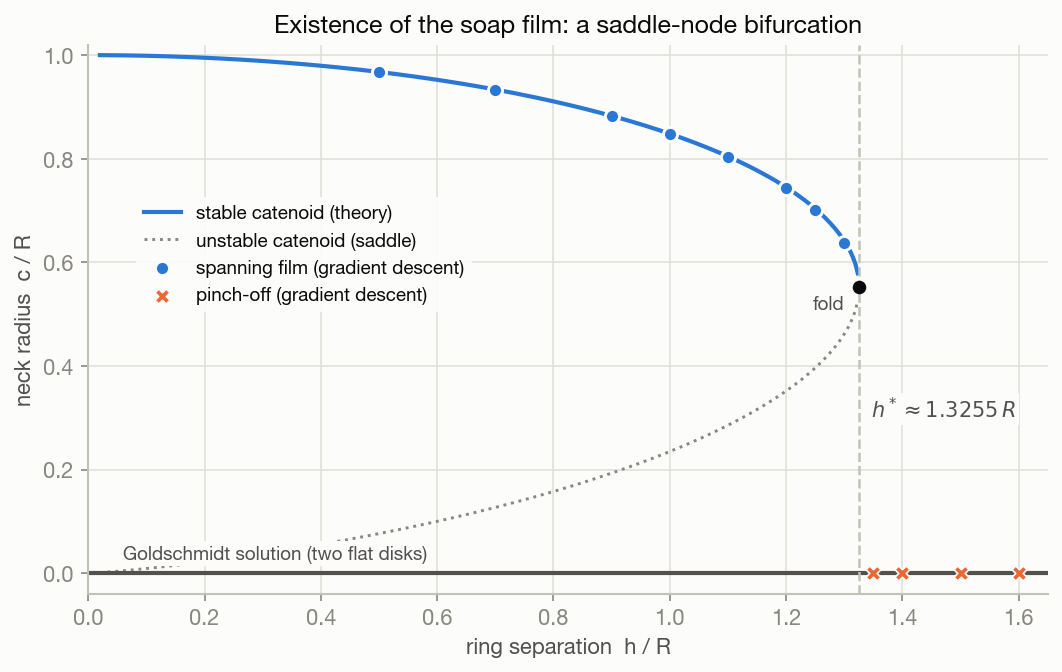
\includegraphics[width=0.72\textwidth]{fig3_bifurcation.png}
\caption{The saddle-node bifurcation of the two-ring soap film. Solid: stable
catenoid branch; dotted: unstable saddle branch; the branches merge at the fold
\eqref{eq:fold} and annihilate. Markers: final neck radius of each gradient
descent run --- on the stable branch below $h^{*}$, at zero (pinch-off,
Goldschmidt) above it.}
\label{fig:bif}
\end{figure}

\section{Discussion}

Three features of the experiment deserve emphasis.

\emph{The right gradient makes the physics automatic.} No curvature was ever
computed: the scheme only differentiates the elementary formula
$\operatorname{area}=\tfrac12\lvert(b-a)\times(c-a)\rvert$. That this descent
is mean curvature flow --- and therefore inherits its qualitative theory:
monotone area, convergence to stable minimal surfaces, finite-time neck
singularities --- is the discrete shadow of the first-variation formula, via
the identity between the summed area gradient and the cotangent Laplacian
applied to the coordinates \cite{pinkall,meyer}.

\emph{The bifurcation is visible in the dynamics, not just the statics.}
Near $h^{*}$ the spectral gap of the stability operator closes, and the flow
exhibits textbook critical slowing-down: at $h/R=1.35$ the neck drifts slowly
for thousands of iterations before the pinch accelerates, while at $h/R=1.5$
collapse is fast. Conversely the growth of the deviation column in
Table~\ref{tab:sweep} toward the fold is the static face of the same
flattening landscape.

\emph{What the discrete flow cannot do is also instructive.} With fixed
connectivity the flow stops at the incipient pinch instead of continuing past
the singularity to the two disks; continuing through topology change is
precisely what measure-theoretic weak formulations (Brakke flow) and
remeshing-based tools such as the Surface Evolver \cite{brakke} are built for.
Our collapse detector is thus an honest declaration of the model's boundary,
not a numerical failure --- and its firing point coincides with the
theoretical non-existence region to within one grid point of the sweep.

\section{Outlook}

The same forty lines of core solver generalize in directions that map onto the
later units of this course: replacing the ring boundary by a disk-topology mesh
over an Enneper-type wire frame probes non-uniqueness for a genuinely
three-dimensional boundary; swapping explicit descent for the
Pinkall--Polthier iteration \cite{pinkall} (solve $\Delta_\Sigma x=0$ with
cotangent weights per step) trades many cheap steps for few linear solves; and
replacing area by the Willmore energy $\int H^{2}$ changes the flow's character
entirely. Finally, the converged meshes and the closed-form branch $c(h)$
constitute a compact, exactly-labelled dataset against which learned solvers
--- e.g.\ physics-informed networks for the minimal surface equation --- can be
benchmarked in later projects.

\begin{thebibliography}{9}\small

\bibitem{euler} L.~Euler,
\emph{Methodus inveniendi lineas curvas maximi minimive proprietate
gaudentes}, Lausanne \& Geneva, 1744.

\bibitem{goldschmidt} C.\,W.\,B.~Goldschmidt,
\emph{Determinatio superficiei minimae rotatione curvae data duo puncta
jungentis circa datum axem ortae}, G\"ottingen, 1831.

\bibitem{plateau} J.~Plateau,
\emph{Statique exp\'erimentale et th\'eorique des liquides soumis aux seules
forces mol\'eculaires}, Gauthier-Villars, Paris, 1873.

\bibitem{rado} T.~Rad\'o,
On Plateau's problem, \emph{Ann.\ of Math.}\ \textbf{31} (1930), 457--469.

\bibitem{douglas} J.~Douglas,
Solution of the problem of Plateau, \emph{Trans.\ Amer.\ Math.\ Soc.}\
\textbf{33} (1931), 263--321.

\bibitem{brakke} K.\,A.~Brakke,
The Surface Evolver, \emph{Experiment.\ Math.}\ \textbf{1} (1992), 141--165.

\bibitem{pinkall} U.~Pinkall and K.~Polthier,
Computing discrete minimal surfaces and their conjugates,
\emph{Experiment.\ Math.}\ \textbf{2} (1993), 15--36.

\bibitem{meyer} M.~Meyer, M.~Desbrun, P.~Schr\"oder, and A.\,H.~Barr,
Discrete differential-geometry operators for triangulated 2-manifolds, in
\emph{Visualization and Mathematics III}, Springer, 2003, 35--57.

\bibitem{dhs} U.~Dierkes, S.~Hildebrandt, and F.~Sauvigny,
\emph{Minimal Surfaces}, 2nd ed., Grundlehren der mathematischen
Wissenschaften 339, Springer, 2010.

\end{thebibliography}

\end{document}
